\section{Introduction}
\label{sec:int}
In this project, we will learn how to measure the performance of an operating system using various user- and system-level operations. Based on prior knowledge of hardware performance as well as measured software behavior, we will approximately estimate the overhead at the operating system level of the whole system hardware/software stack. We select a well-known multi-user time-sharing operating system, Ubuntu 14.04.1 LTS (desktop) \footnote{http://www.ubuntu.com/download/desktop}, as our experiment platform. This is a long time supported Linux distribution with stable performance and reliable system functions. Our hardware platform is a $Lenovo Y400$  workstation equipped with an $Intel$  $4 cores$ processor. The experimental results indicate that our system configuration is trustable, it also helps us understand the underlying mechanisms of the system as a good reference, which interacts with both software from upper-layer and hardware from lower-layer.
In this project, our major achievement is on the design of experiments (DOE), prediction of performance and analysis on the performance gap between predictive and measured ones. We implement our ideas of DOE by $C$ programming to verify how the system and user operations will impact the performance. We use $gcc$ as the major compiler for our experiments, with all optimization options turned off in the Makefiles. Optimization options intentionally changes code sections to pursue performance gain, which unintentionally disables our desired operations and effect of measurement. As a result, most of our programs are expected to be directly compiled (or, ``interpreted'') in a compiler's perspective.
This project constructs an impressive structure of computing system, in which the operating system plays an role of administrator and coordinator between the application requests and device supports. We are able to effectively analyze an operating system, identify major features of design, advantages and disadvantages, and most importantly, how this middle layer of coordinator impacts the overall performance of the whole stack and how we could possibly improve it based on our accumulated experiences on it.

\subsection{Tasks Allocation}
\chunbin{Xun will conduct the  CPU experiments, and  Chunbin will conduct the Memory experiments. Jiapeng will conduct the File system experiments. We will work together to finish the Network experiments.}

We will spend about 90 hours on this project in total (10 hours per week, and we will use 9 weeks) including the time on reading related papers.

\section{Machine Description}
\label{sec:pc}
All the experiments that we conducted are on the machine and the system, which is characterized in Table \ref{tab:pc}.
This is a $Lenovo Y400$ desktop 64bit machine manufactured. It has a wired network connection to the local area network gated by $137.110.161.79$ located in the office $3232$, CSE department. The operating system running on it is an Ubuntu 14.04.1 LTS desktop.
Notice that we include some basic hardware performance numbers of machine components which are obtained from the manufacturer's datasheets, e.g., I/O bus operating speed, etc. These numbers facilitate our raw performance estimation of running the applications on the stacked layers. These numbers will be frequently referred to in our overhead measurement during the following sections.

%\begin{comment}
%\begin{figure}
%\centering
%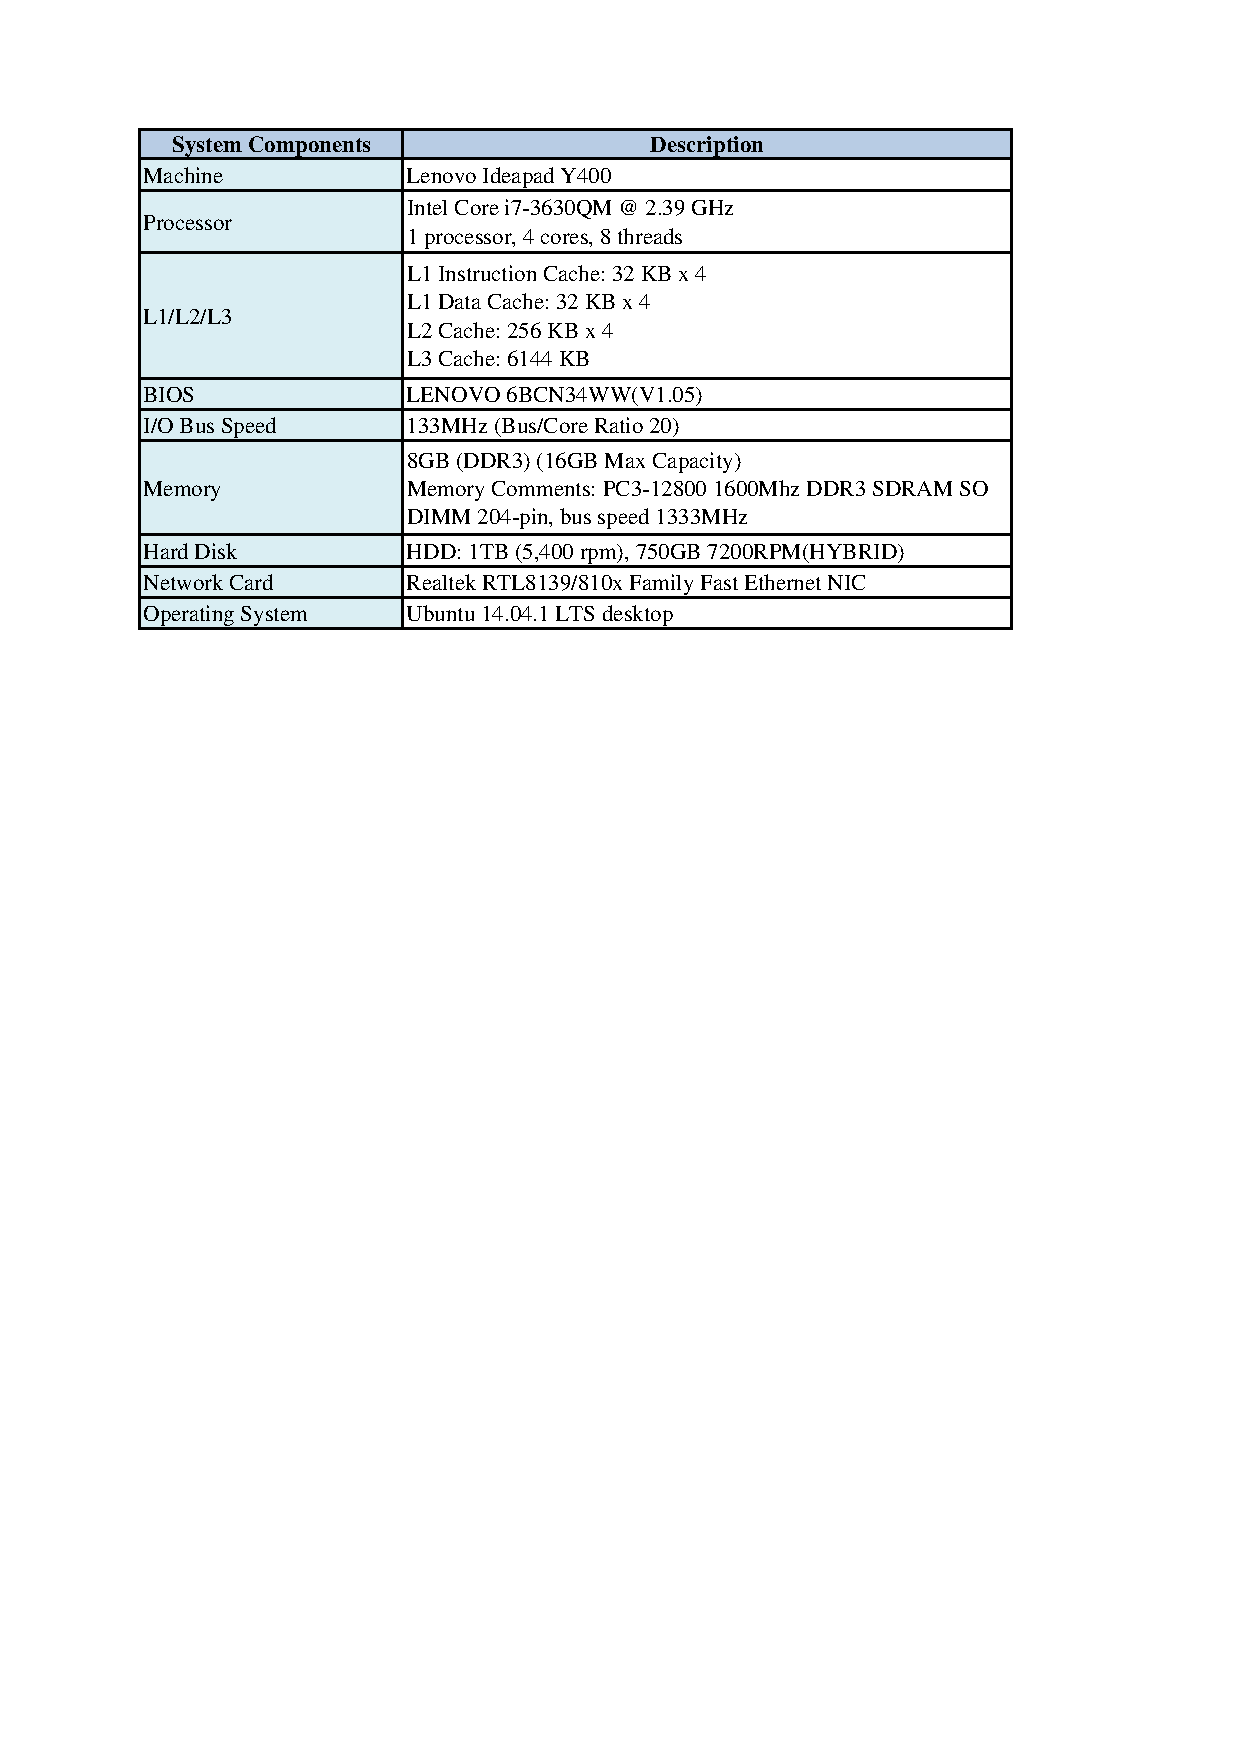
\includegraphics[width=0.4\columnwidth, angle=0]{./figs/Machine_Description.pdf}
%\caption{Machine Description of Lenovo Y400.}
%\end{figure}
%\end{comment}

\begin{figure}[!htp]
\centering
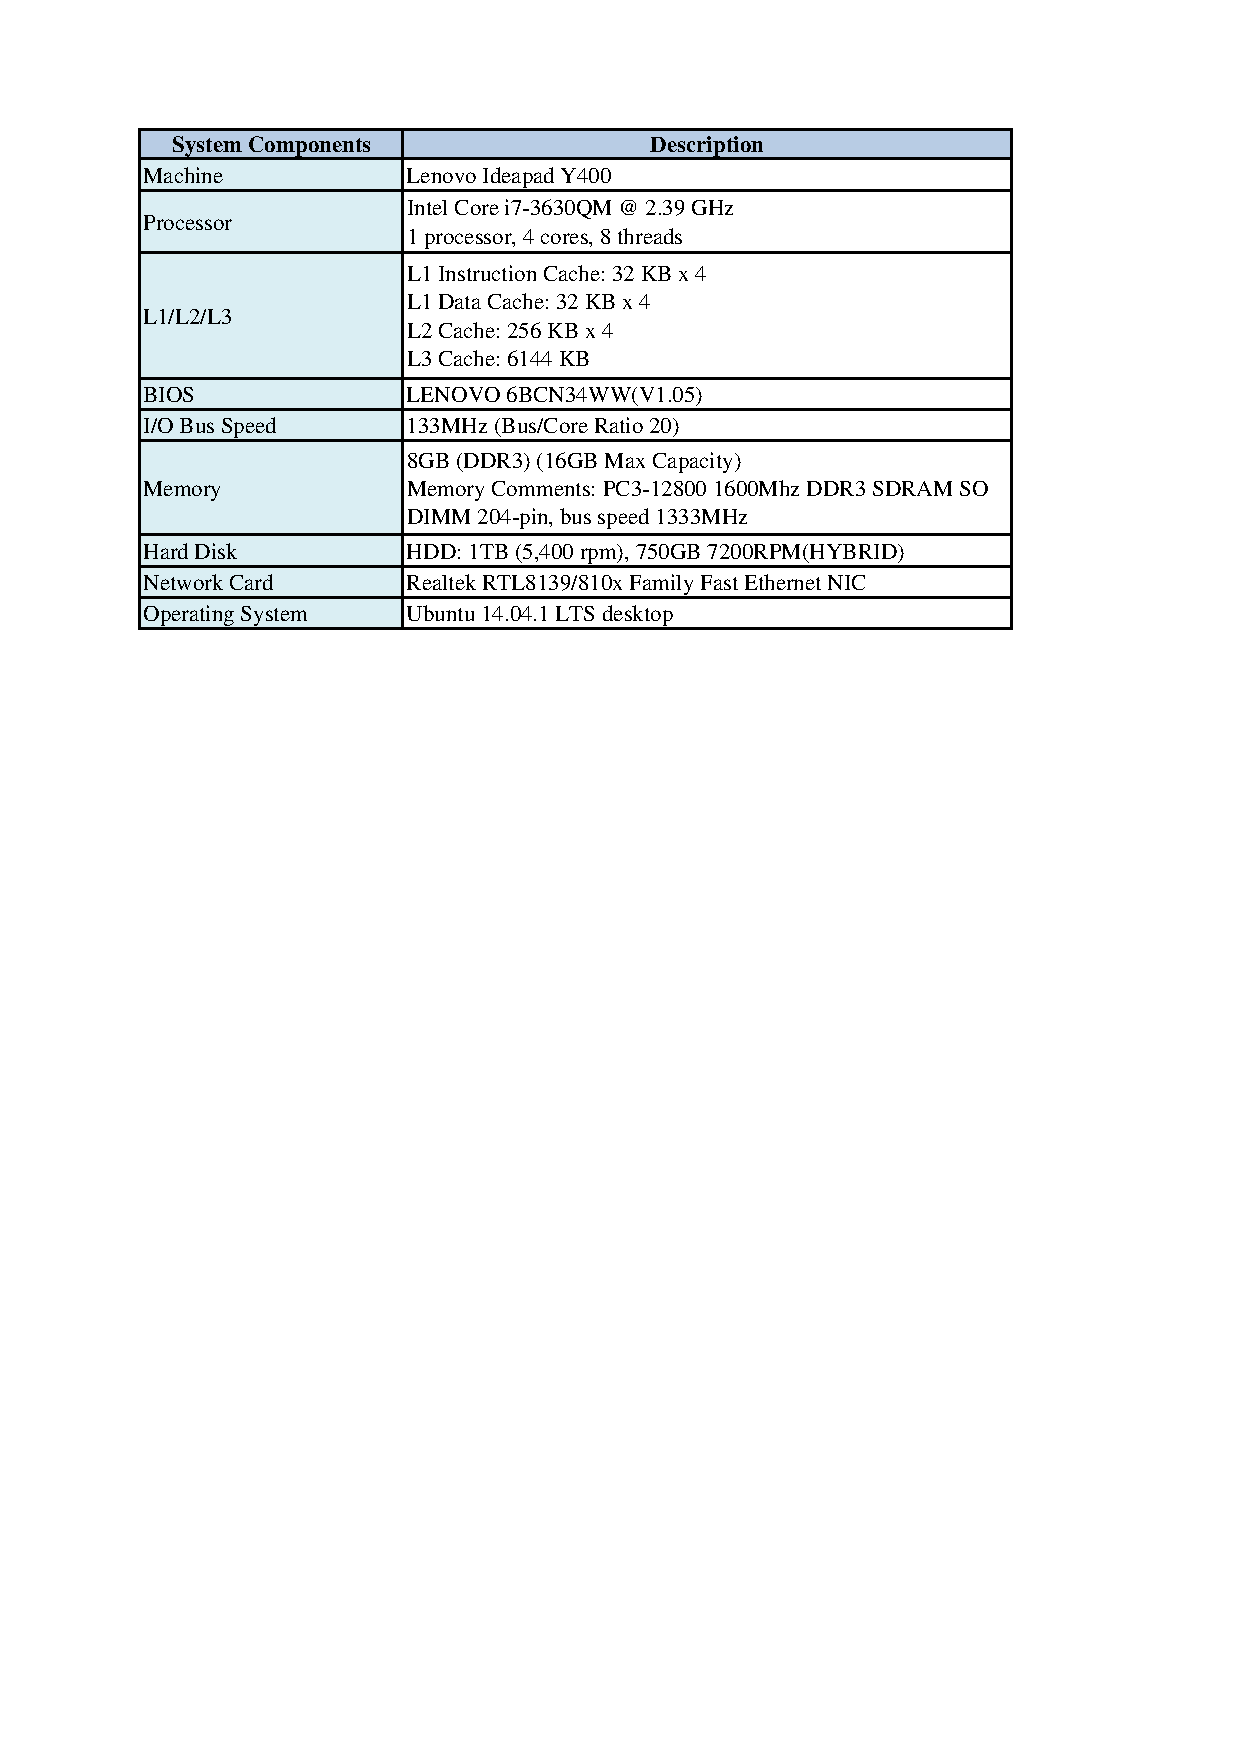
\includegraphics[width=0.5\textwidth]{figs/Machine_Description.pdf}
 \caption{Machine Description of Lenovo Y400.}
\end{figure}


\section{CPU, Scheduling, and OS Services }
\label{sec:cpu}
In this section we design several experiments to measure the performance of operations related to on-chip processor scheduling. Our experiments will provide a couple of measured results of interests.
\subsection{Measurement overhead}
\chunbin{Measurement overhead: Report the overhead of reading time, and report the overhead of using a loop to measure many iterations of an operation.}

\subsection{Procedure call overhead}
\chunbin{Procedure call overhead: Report as a function of number of integer arguments from 0-7. What is the increment overhead of an argument?}

\subsection{system call overhead}
\chunbin{System call overhead: Report the cost of a minimal system call. How does it compare to the cost of a procedure call? Note that some operating systems will cache the results of some system calls (e.g., idempotent system calls like getpid), so only the first call by a process will actually trap into the OS.}

\subsection{Task creation time}
\chunbin{Task creation time: Report the time to create and run both a process and a kernel thread. How do they compare?}

\subsection{Context switch time}
\chunbin{Context switch time: Report the time to context switch from one process to another, and from one kernel thread to another. How do they compare? In the past students have found using blocking pipes to be useful for forcing context switches}

\end{document}

